%!TEX root = main.tex
\section{Data}

To estimate the run-time of a CAL module execution, we created a machine learning model for each module. With each run of the module (within some application of the Baltic LSC system), we will get another data point to train our model. The following features (explanatory variables)  make up the input data set for a model:

\begin{enumerate}
	\item CPUs limit - called \textit{mili-cores} - the fraction of a physical CPU used to carry out the module execution.
	\item The total size of an input data in bytes.
	\item The largest element size of an input data (if the input data is a set of files type, it is the largest size of a file within the set).
	\item The average size of an input element.
	\item The number of input data elements.
\end{enumerate}

The last three features make clear sense only if input data is a set of files. Otherwise, if data is just a single file, the features can be a sort of data features representation carrying more detailed information about the data than only a total size. For the data frame, the number of input elements can be equal to the number of columns. The max element size will be a quotient of the total size and the number of columns, and the average size will be equal to that quotient as well.  In other cases (other kinds of input data), one can prepare specific, additional features and store their values for each execution (to enable their use for training in the future).  In this work, we simplified the task to the features mentioned above. Our dependent value (that we are going to estimate) is an execution time of a module. 

We created two CAL applications based on four modules with different types of input data. The first application (consisting of three modules) takes the movie as input data, marks people's faces on each frame, and then returns the movie with marked people faces as output data. The second one consists of just a single module, and it searches the best hyperparameters of XGBoost algorithm within the parameters grid. Table~\ref{tab:modules} describe the modules that we used in the research. For each module, we created a set of 10 different input data. Next, we ran the modules with the all mentioned data sets using various CPU resources (from 0.5 CPUs up to 4.0 CPUs with 0.5 step). Finally, we received the data frame with the number of 4 (number of modules) * 8 (different CPUs resources) * 10 (number of input data sets) = 320 rows that we used to train and validate our models. Part of the models' input data is presented in Table~\ref{tab:example_df}. 

\begin{figure*}[!t]
	\centering
	\begin{minipage}{0.75\linewidth}
		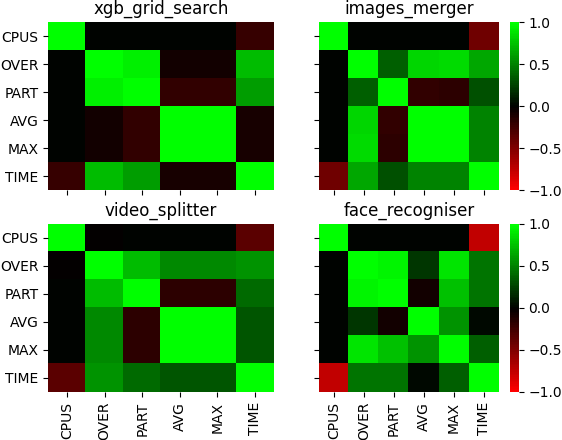
\includegraphics[width=1.0\textwidth]{corr}
	\end{minipage}
	\caption{Data columns Spearman`s correlation per module.}
	\label{fig:corr}
\end{figure*}

\begin{figure*}[!t]
	\centering
	\begin{minipage}{0.75\linewidth}
		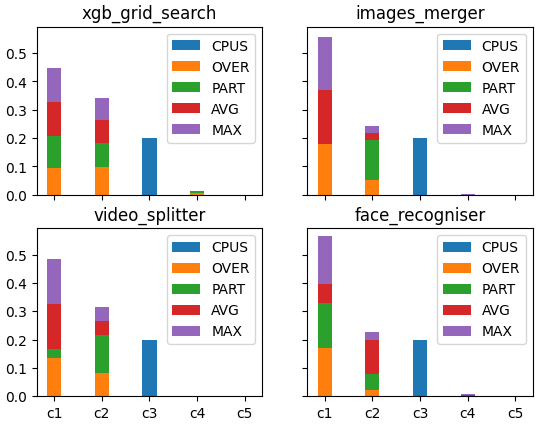
\includegraphics[width=1.0\textwidth]{pca_importance}
	\end{minipage}
	\caption{PCA importance per module.}
	\label{fig:pca}
\end{figure*}

\begin{table*}[!t]
	\centering
	\caption{\label{tab:example_df}Part of the data frame for models training and validation.}
	\begin{minipage}{0.9\linewidth}
		{\footnotesize
			\begin{tabular}{|c c c c c c >{\columncolor[gray]{0.9}}c|} 
				\hline
				Module ID & mCPUs & total size [B] & number of elements & max size [B] & average size [B] & time [s] \\ [0.5ex] 
				\hline\hline
				1 & 4.0 & 1703379 & 544 & 3131 & 3131 & 3.909 \\ 
				\hline
				1 & 4.0 & 809881 & 548 & 1477 & 1477 & 1.981  \\
				\hline
				1 & 4.0 & 1711796 & 1392 & 1229 & 1229 & 11.371 \\
				\hline
				... & ... & ... & ... & ... & ... & ... \\ [1ex] 
				\hline
			\end{tabular}
		}
	\end{minipage}
\end{table*}	

To make the models' data more understandable, we prepared two figures that show interactions between the features. Figure~\ref{fig:corr} shows how each column of the dataset is correlated with the other ones (green indicates positive correlation, red indicates negative correlation). As a correlation coefficient between two columns, we used Spearman's rank correlation coefficient. As we can see, the data-based input features are mostly positively correlated with each other to some point, and they obviously are positively correlated with the run-time as well. The CPUs feature is negatively correlated with the run-time for each module (highest correlation for \textit{face\_recogniser}). As the data-based input features are so strongly correlated, we performed the PCA analysis to determine how the specif column affects the input data variation. Figure~\ref{fig:pca} shows the results.  The only environment-based feature, CPUs, is not correlated with other ones and impacts the data variation with a value equal to 1/(number of columns) = 0.2 for each module. The rest of the variance falls on data-based features. The PCA analysis shows that we could compress our input data to only three features and still keep almost all variance (the same situation for each module). We kept the original input data for more clearness, but one should consider dimensionality reduction if he has decided to provide many columns.

\begin{table}[hbt!]
	\centering
	\caption{\label{tab:modules}Modules that we used in the research.}
	\begin{tabular}{|c c c|} 
		\hline
		ID (APP ID) & Name & Input data \\ [0.5ex] 
		\hline\hline
		1(1) & video\_splitter & video file \\ 
		\hline
		2(1) & face\_recogniser & image files \\
		\hline
		3(1) & images\_merger & image files \\
		\hline
		4(2) & xgb\_grid\_search & CSV file \\
		\hline
	\end{tabular}
\end{table}
